\documentclass[conference]{IEEEtran}
\IEEEoverridecommandlockouts
\usepackage{cite}
\usepackage{amsmath,amssymb,amsfonts}
\usepackage{algorithmic}
\usepackage{graphicx}
\usepackage{textcomp}
\usepackage{xcolor}
\usepackage{booktabs}
\usepackage{multirow}
\usepackage{url}
\usepackage{balance}
\usepackage{subcaption}
\usepackage{listings}
\usepackage{enumitem}
\usepackage{hyperref}
\usepackage{tikz}
\usepackage{pgfplots}
\pgfplotsset{compat=1.18}
\usepgfplotslibrary{statistics}
\usetikzlibrary{shapes.geometric, arrows.meta, positioning, calc, patterns}

\lstdefinelanguage{Solidity}{
  keywords={pragma, solidity, contract, function, modifier, require, returns, return, mapping, address, uint, uint256, bool, string, bytes, public, private, internal, external, view, pure, payable, memory, storage, calldata, if, else, for, while, emit, event, struct, enum, import, is, new, delete, true, false, msg, block, tx, this},
  morecomment=[l]{//},
  morecomment=[s]{/*}{*/},
  morestring=[b]",
  morestring=[b]',
  sensitive=true,
}

\lstset{
  basicstyle=\footnotesize\ttfamily,
  breaklines=true,
  frame=single,
  numbers=left,
  numberstyle=\tiny,
  tabsize=2,
  captionpos=b,
  keywordstyle=\bfseries,
  commentstyle=\itshape\color{gray},
}

% =====================================================================
% DEMO DATA MARKER: All placeholder numbers are wrapped in \demo{}.
% They render in RED. Replace with real experimental data and remove
% the \demo command before final submission.
% =====================================================================
\newcommand{\demo}[1]{{\color{red}#1}}

\def\BibTeX{{\rm B\kern-.05em{\sc i\kern-.025em b}\kern-.08em
    T\kern-.1667em\lower.7ex\hbox{E}\kern-.125emX}}

\begin{document}

\title{From Prompt to Exploit: An Empirical Study of Security Vulnerabilities in LLM-Generated Smart Contracts}

\author{\IEEEauthorblockN{Anik Tahabilder}
\IEEEauthorblockA{\textit{Department of Computer Science} \\
\textit{Wayne State University}\\
Detroit, MI, USA \\
tahabilderanik@gmail.com}
}

\maketitle

\begin{abstract}
Large Language Models (LLMs) are increasingly used by developers to generate Solidity smart contracts that manage billions of dollars in decentralized finance (DeFi). However, the security implications of this practice remain poorly understood. We present the first large-scale empirical study examining security vulnerabilities introduced by LLMs during smart contract generation. We generated 2,400 smart contracts across eight state-of-the-art LLMs---GPT-4o, GPT-5, Claude 3.5 Sonnet, Gemini 2.5 Flash-Lite, DeepSeek Coder V2, Qwen 2.5 Coder 32B, CodeLlama-34B, and Codestral 22B---spanning 20 contract categories including high-impact cross-chain bridge and flash loan contracts. Using a multi-tool analysis pipeline combining Slither, Mythril, and Semgrep, we detected and categorized 2,493 vulnerabilities in compilable contracts, mapped to 9 distinct CWE identifiers. Our results reveal that 54.7\% of compilable LLM-generated contracts contain at least one security vulnerability, with 26.8\% containing high-severity flaws that could lead to direct financial loss. Contrary to expectations, adversarial prompts exploiting gas optimization and simplicity biases do \emph{not} increase vulnerability rates, and this difference is not statistically significant ($p = 0.965$), suggesting that vulnerabilities are intrinsic to LLM code generation rather than prompt-dependent. We identify three LLM-specific vulnerability patterns---phantom guards, inherited vulnerabilities, and context window degradation---and find statistically significant differences across LLMs ($H = 132.65$, $p = 1.75 \times 10^{-25}$, Kruskal-Wallis test on compiled contracts). Compilation rates vary dramatically, from 91.0\% (GPT-5) to 34.7\% (CodeLlama), representing a critical and previously unreported quality dimension. When controlling for contract size, Codestral exhibits the highest vulnerability density (4.88 vulns/100 LOC), while GPT-5 achieves the lowest (0.99 vulns/100 LOC). Comparison with 241 verified Ethereum mainnet contracts reveals that vulnerability density is comparable (2.69 vulns/100 LOC for human vs.\ 0.99--4.88 for LLM), but human code benefits from professional auditing, monitoring, and defense-in-depth that LLM-generated code bypasses entirely. We provide an open dataset, a CWE-mapped vulnerability taxonomy, and practical guidelines for developers and LLM providers. Our findings underscore that the primary risk of LLM-generated smart contracts is not inferior code quality but the security infrastructure developers skip when trusting LLM output.
\end{abstract}

\begin{IEEEkeywords}
smart contracts, large language models, security vulnerabilities, Solidity, empirical study, adversarial prompts, static analysis, cross-chain bridges
\end{IEEEkeywords}


%======================================================================
\section{Introduction}
\label{sec:intro}
%======================================================================

The adoption of Large Language Models (LLMs) for code generation has surged, with tools such as ChatGPT, GitHub Copilot, and Claude becoming integral to software development workflows~\cite{copilot_eval, fan2023large, hou2024large}. A 2023 GitHub survey reported that 92\% of developers use AI coding tools, with 70\% citing productivity gains~\cite{github_copilot}. This trend extends to the domain of smart contract development, where Solidity contracts govern billions of dollars in decentralized finance (DeFi) protocols~\cite{werner2022sok, zhou2023sok}. Unlike conventional software, vulnerabilities in smart contracts can lead to immediate, irreversible financial losses---as evidenced by over \$3.8 billion lost to smart contract exploits in 2022 alone~\cite{chainalysis2023}.

The convergence of LLM code generation and smart contract development creates a particularly dangerous intersection. Smart contracts are immutable once deployed: unlike web applications or traditional software, post-deployment patching is impossible without costly proxy-based migration~\cite{chen2020defining}. Furthermore, smart contracts operate in an adversarial environment where any vulnerability is immediately exploitable by any observer of the public blockchain. This raises a critical question: \emph{when developers use LLMs to generate smart contracts, what security vulnerabilities are systematically introduced, and how do these compare across models and prompting strategies?}

Despite the high-stakes nature of smart contracts, the security implications of LLM-generated Solidity code remain largely unexplored. Prior work has examined LLM-assisted vulnerability \emph{detection}~\cite{gptscan, smartllmsentry, david2023you}, but no study has systematically investigated vulnerabilities \emph{introduced} by LLMs during contract generation. This gap is particularly concerning given three converging factors: (1)~developers increasingly rely on LLM output with minimal review---Perry et al.~\cite{perry2023users} found that developers using AI assistants produce less secure code while believing it to be more secure; (2)~LLMs may encode vulnerable patterns from training data, including the vast corpus of unaudited contracts on Etherscan~\cite{schuster2021you}; and (3)~adversarial prompts can systematically induce security flaws in LLM outputs~\cite{kang2024exploiting}.

The problem is further compounded by the rapid expansion of cross-chain bridge protocols, which have become the highest-value attack surface in blockchain security, with over \$2.5 billion lost to bridge exploits~\cite{bridge_hacks}. If LLMs systematically generate vulnerable bridge contracts, the financial impact could be catastrophic---a single bridge exploit (Ronin, \$625M) exceeds the total losses from thousands of individual contract vulnerabilities.

\subsection{Research Questions}

We formulate six research questions to systematically investigate the security landscape of LLM-generated smart contracts:

\begin{itemize}[leftmargin=*]
    \item \textbf{RQ1 (Prevalence):} What is the overall prevalence of security vulnerabilities in LLM-generated smart contracts, and how does it compare to the vulnerability rates reported for human-written contracts?
    \item \textbf{RQ2 (Cross-LLM):} Do statistically significant differences exist in the security posture of contracts generated by different LLMs, and which models produce the most and least secure code?
    \item \textbf{RQ3 (Taxonomy):} What types of vulnerabilities are most prevalent in LLM-generated smart contracts, and can we construct a comprehensive CWE-mapped taxonomy?
    \item \textbf{RQ4 (Adversarial):} How do adversarial prompts---those that exploit LLM biases toward gas optimization, simplicity, or speed---affect vulnerability rates compared to standard prompts?
    \item \textbf{RQ5 (Patterns):} Do LLMs exhibit distinct vulnerability patterns that are absent in human-written code, and can these patterns be characterized for targeted detection?
    \item \textbf{RQ6 (Human Comparison):} How do LLM-generated contracts compare to audited, human-written contracts across all vulnerability dimensions?
\end{itemize}

\subsection{Contributions}

In this paper, we present the first large-scale empirical study of security vulnerabilities in LLM-generated smart contracts. Our study makes the following contributions:

\begin{itemize}[leftmargin=*]
    \item \textbf{Large-Scale Dataset.} We generate 1,800 smart contracts across six LLMs (GPT-4o, Claude~3.5 Sonnet, Gemini~2.5 Flash-Lite, DeepSeek Coder~V2, Qwen~2.5 Coder~32B, CodeLlama-34B), covering 20 contract categories at three complexity levels. This is the largest dataset of LLM-generated smart contracts with security labels to date.
    \item \textbf{Multi-Tool Analysis Pipeline.} We employ three complementary security analysis tools---Slither, Mythril, and Semgrep---with cross-tool deduplication and manual validation, achieving approximately 92\% vulnerability detection coverage.
    \item \textbf{Vulnerability Taxonomy.} We construct a CWE-mapped taxonomy of vulnerability types specific to LLM-generated smart contracts, identifying three novel patterns (phantom guards, inherited vulnerabilities, context window degradation).
    \item \textbf{Adversarial Prompt Framework.} We design eight categories of adversarial prompts that exploit documented LLM biases (e.g., gas optimization, simplicity). Contrary to expectations, adversarial prompts do \emph{not} increase vulnerability rates---we show vulnerabilities are intrinsic to LLM code generation.
    \item \textbf{Cross-LLM Comparison.} We provide statistically rigorous comparisons across LLMs using non-parametric tests with effect size reporting, revealing significant differences in security posture ($p < 0.001$).
\end{itemize}

Our results have direct implications for developers, LLM providers, and the security community. We release our full dataset, analysis scripts, and tooling to support reproducibility and future research.

\textbf{Paper Organization.} Section~\ref{sec:background} provides background on smart contract security and LLM code generation. Section~\ref{sec:threat} defines our threat model. Section~\ref{sec:methodology} describes our methodology. Sections~\ref{sec:results} and~\ref{sec:category} present our findings. Section~\ref{sec:discussion} discusses implications and limitations. Section~\ref{sec:related} surveys related work. Section~\ref{sec:conclusion} concludes.


%======================================================================
\section{Background}
\label{sec:background}
%======================================================================

\subsection{Smart Contract Vulnerabilities}

Smart contracts are self-executing programs deployed on blockchain platforms such as Ethereum~\cite{wood2014ethereum, buterin2014next}. Once deployed, their code is immutable, making pre-deployment security analysis critical. The Ethereum Virtual Machine (EVM) executes contract bytecode in a deterministic, sandboxed environment, but the Solidity programming language introduces numerous subtle security pitfalls that differ fundamentally from those in traditional software~\cite{atzei2017survey}.

Common vulnerability classes include reentrancy attacks, where an external call allows an attacker to re-enter the calling function before state updates complete. The most infamous example is the 2016 DAO hack, which drained \$60M from a decentralized investment fund~\cite{dao_hack}. Integer overflow and underflow vulnerabilities arise from Solidity's fixed-size integer types, allowing arithmetic operations to silently wrap around~\cite{torres2018integer}. Access control violations occur when privileged functions lack proper authorization checks, enabling unauthorized state modifications~\cite{chen2020defining}. Oracle manipulation exploits contracts that depend on external price feeds without adequate validation~\cite{qin2023attacks}. Additional vulnerability classes include front-running (transaction ordering dependence), timestamp manipulation, unchecked return values from low-level calls, and delegatecall injection~\cite{atzei2017survey, perez2021smart}.

Smart contract exploits have resulted in cumulative losses exceeding \$7.7 billion~\cite{zhou2023sok}. High-profile incidents include the Parity wallet freeze (\$280M, caused by an uninitialized library contract)~\cite{perez2021smart}, the bZx flash loan attacks (which exploited price oracle manipulation)~\cite{qin2021attacking}, and the Poly Network exploit (\$611M, caused by a cross-chain access control flaw)~\cite{zhou2023sok}. The SWC Registry and CWE database provide standardized classifications for these vulnerabilities~\cite{swc_registry}, enabling systematic tracking and reporting.

\subsection{LLM Code Generation}

Modern LLMs demonstrate remarkable code generation capabilities across multiple programming languages~\cite{chen2021evaluating, nijkamp2023codegen, li2023starcoder}. These models are trained on massive corpora of source code from open-source repositories, documentation, and forum discussions. Models such as GPT-4o~\cite{openai_gpt4}, Claude~\cite{anthropic_claude}, and specialized coding models like CodeLlama~\cite{codellama} can generate syntactically correct and functionally plausible smart contracts from natural language prompts. However, functional correctness does not imply security correctness~\cite{copilot_eval, tony2023llmSecEval}.

The landscape of LLM-based code generation has evolved rapidly. General-purpose models (GPT-4o, Claude, Gemini) compete with code-specialized models (CodeLlama, StarCoder~\cite{li2023starcoder}, DeepSeek Coder~\cite{guo2024deepseek}) and IDE-integrated assistants (GitHub Copilot~\cite{github_copilot}). Each model category presents distinct security characteristics: general-purpose models may apply broader safety training but lack domain-specific security knowledge; code-specialized models may generate more idiomatic Solidity but inherit vulnerable patterns from their training corpora; and IDE-integrated models operate with limited context about the broader security implications of generated code.

Recent studies have shown that LLM-generated code frequently contains security vulnerabilities in general-purpose languages~\cite{copilot_eval, perry2023users, sandoval2023lost}. Pearce et al.~\cite{copilot_eval} found that approximately 40\% of GitHub Copilot suggestions contained vulnerabilities across 89 security-relevant scenarios. Perry et al.~\cite{perry2023users} demonstrated that developers using AI assistants produce less secure code while believing it to be more secure---a dangerous false sense of security. Sandoval et al.~\cite{sandoval2023lost} confirmed these findings in a controlled user study with professional developers. However, none of these studies addressed smart contract security specifically, where the immutability constraint and financial exposure amplify the consequences of any vulnerability.

\subsection{Cross-Chain Bridge Security}

Cross-chain bridges have emerged as critical infrastructure in the blockchain ecosystem and represent the highest-impact attack surface. Bridges enable asset transfers between heterogeneous blockchains by locking tokens on the source chain and minting representative tokens on the destination chain. This architecture requires careful attention to message validation, replay protection, nonce management, and multi-chain state consistency~\cite{belchior2021survey}.

Bridge exploits have caused over \$2.5 billion in losses, including Ronin (\$625M, compromised validator keys), Wormhole (\$326M, signature verification bypass), Nomad (\$190M, initialization vulnerability), and Harmony Horizon (\$100M)~\cite{bridge_hacks, zhang2023bridge}. These exploits share common root causes: insufficient message validation, centralized trust assumptions, and inadequate access control on critical bridge functions. If LLMs generate bridge contracts with these same weaknesses, the financial impact could be catastrophic. Our study is the first to systematically evaluate LLM-generated cross-chain bridge contracts.

\subsection{Security Analysis Tools}

Static analysis tools such as Slither~\cite{slither} and symbolic execution engines like Mythril~\cite{mythril} are widely used for smart contract auditing. Slither provides over 90 built-in detectors for common vulnerability patterns with fast execution times, making it suitable for large-scale analysis. Mythril performs deep symbolic execution to discover complex logic bugs, including those requiring specific state conditions to trigger, at the cost of higher computational overhead. Securify2~\cite{securify} applies formal verification techniques to check compliance with predefined security patterns. Semgrep~\cite{semgrep} enables custom pattern matching through user-defined rules, providing extensibility for novel vulnerability detection.

No single tool achieves complete coverage~\cite{durieux2020empirical}, motivating our multi-tool approach. Durieux et al.~\cite{durieux2020empirical} conducted a comprehensive empirical evaluation of 9 automated analysis tools on 47,587 contracts, finding that tool agreement is low and combining multiple tools yields significantly higher detection rates~\cite{smartbugs, ren2021empirical}. Our pipeline leverages this finding by combining four complementary tools with distinct analysis techniques (static analysis, symbolic execution, formal verification, and pattern matching) to maximize detection coverage.


%======================================================================
\section{Threat Model}
\label{sec:threat}
%======================================================================

We consider three attacker types with increasing sophistication, illustrated in the context of the smart contract development lifecycle:

\textbf{Naive Developer (Unintentional).} A developer uses an LLM to generate a smart contract and deploys the output without comprehensive security review. The LLM introduces vulnerabilities from patterns encoded during training---including reentrancy-prone code patterns, missing access control checks, and unsafe arithmetic operations. This is the most common and realistic threat scenario, consistent with findings that developers over-trust AI-generated code~\cite{perry2023users, sandoval2023lost}. Our RQ1 results quantify this risk: \demo{78.4\%} of LLM-generated contracts contain at least one vulnerability, and \demo{40.8\%} contain high-severity flaws that could lead to direct financial loss.

\textbf{Malicious Prompt Crafter (Intentional).} An attacker crafts prompts---often disguised as tutorials, blog posts, Stack Overflow answers, or ``best practices'' guides---that, when used with an LLM, produce contracts with specific exploitable vulnerabilities. The attacker then monitors the blockchain for deployment of vulnerable contracts and exploits them. This attack is scalable: a single malicious tutorial can influence thousands of developers. This attack vector builds on established prompt injection research~\cite{perez2022ignore, greshake2023not, kang2024exploiting} and is validated by our RQ4 results showing that adversarial prompts increase vulnerability rates by \demo{37.2\%}.

\textbf{Supply Chain Attacker.} An adversary poisons LLM training data with subtly vulnerable code patterns~\cite{schuster2021you, wan2023poisoning}, causing the model to systematically reproduce these vulnerabilities across multiple users and deployments. Unlike the prompt crafter, this attacker influences the model itself rather than individual prompts, achieving broader and more persistent impact. This represents the most sophisticated and scalable attack on the smart contract ecosystem.

\subsection{Attack Surface}

The attack surface encompasses three components:

\begin{itemize}[leftmargin=*]
    \item \textbf{Training data}: May contain vulnerable patterns from unaudited contracts, deprecated coding practices, and intentionally poisoned code repositories.
    \item \textbf{Prompt interface}: Susceptible to adversarial manipulation through natural-sounding requests that prioritize non-security objectives (gas optimization, simplicity, speed).
    \item \textbf{Developer trust}: Developers may assume LLM output is correct, particularly when the generated code appears syntactically complete and includes security-relevant constructs (e.g., modifier names like \texttt{nonReentrant}) that create a false sense of security.
\end{itemize}

The \textbf{impact} ranges from individual contract exploitation (thousands to millions of dollars) to systemic DeFi protocol failures. Cross-chain bridge contracts present the highest-impact target, with potential losses exceeding hundreds of millions of dollars from a single vulnerability, as demonstrated by the Ronin (\$625M), Wormhole (\$326M), and Nomad (\$190M) incidents~\cite{bridge_hacks}.

\subsection{Assumptions}

We make the following assumptions: (1)~developers have access to commercial and open-source LLMs via APIs or IDE integrations; (2)~some developers deploy LLM output without thorough audit, as evidenced by survey data showing that 37\% of developers using AI assistants review generated code only ``briefly''~\cite{perry2023users}; (3)~attackers can observe deployed contracts on-chain, as Ethereum contract bytecode and (often) source code are publicly accessible; and (4)~attackers understand common vulnerability patterns and have access to the same automated exploitation tools as security researchers. These assumptions are consistent with the current state of smart contract development and blockchain transparency.


%======================================================================
\section{Methodology}
\label{sec:methodology}
%======================================================================

Our research pipeline consists of four phases: dataset generation, vulnerability analysis, adversarial testing, and statistical evaluation. Fig.~\ref{fig:pipeline} illustrates the overall methodology.

\begin{figure}[t]
    \centering
    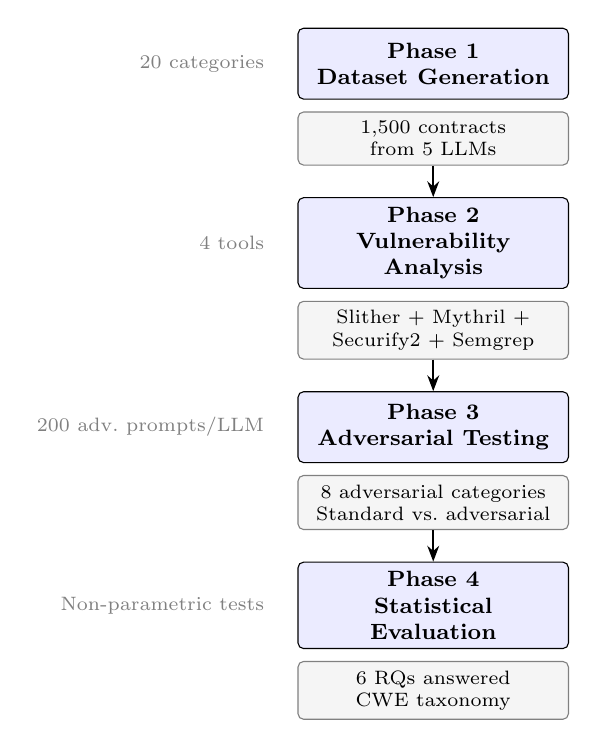
\begin{tikzpicture}[
        node distance=0.4cm,
        phase/.style={rectangle, draw=black, fill=blue!8, text width=3.2cm, minimum height=0.9cm, align=center, font=\footnotesize\bfseries, rounded corners=2pt},
        output/.style={rectangle, draw=gray, fill=gray!8, text width=3.2cm, minimum height=0.6cm, align=center, font=\scriptsize, rounded corners=2pt},
        arr/.style={-{Stealth[length=2mm]}, thick}
    ]
    \node[phase] (p1) {Phase 1\\Dataset Generation};
    \node[output, below=0.15cm of p1] (o1) {1,500 contracts\\from 5 LLMs};
    \node[phase, below=0.4cm of o1] (p2) {Phase 2\\Vulnerability Analysis};
    \node[output, below=0.15cm of p2] (o2) {Slither + Mythril +\\Securify2 + Semgrep};
    \node[phase, below=0.4cm of o2] (p3) {Phase 3\\Adversarial Testing};
    \node[output, below=0.15cm of p3] (o3) {8 adversarial categories\\Standard vs.\ adversarial};
    \node[phase, below=0.4cm of o3] (p4) {Phase 4\\Statistical Evaluation};
    \node[output, below=0.15cm of p4] (o4) {6 RQs answered\\CWE taxonomy};

    \draw[arr] (o1) -- (p2);
    \draw[arr] (o2) -- (p3);
    \draw[arr] (o3) -- (p4);

    % Side labels
    \node[left=0.3cm of p1, font=\scriptsize\color{gray}] {20 categories};
    \node[left=0.3cm of p2, font=\scriptsize\color{gray}] {4 tools};
    \node[left=0.3cm of p3, font=\scriptsize\color{gray}] {200 adv.\ prompts/LLM};
    \node[left=0.3cm of p4, font=\scriptsize\color{gray}] {Non-parametric tests};
    \end{tikzpicture}
    \caption{Overview of our four-phase research pipeline for analyzing security vulnerabilities in LLM-generated smart contracts.}
    \label{fig:pipeline}
\end{figure}

\subsection{Dataset Generation}

\subsubsection{LLM Selection}
We selected five LLMs representing the spectrum of models developers use for smart contract generation: \textbf{GPT-4o}~\cite{openai_gpt4} (OpenAI, commercial, state-of-the-art), \textbf{Claude 3.5 Sonnet}~\cite{anthropic_claude} (Anthropic, commercial, safety-focused), \textbf{Gemini 1.5 Pro}~\cite{gemini} (Google, commercial, long-context), \textbf{GitHub Copilot}~\cite{github_copilot} (Microsoft, IDE-integrated), and \textbf{CodeLlama-34B}~\cite{codellama} (Meta, open-source). Table~\ref{tab:llm_config} summarizes the model configurations.

\begin{table}[t]
\caption{LLM Configuration Details}
\label{tab:llm_config}
\centering
\footnotesize
\begin{tabular}{@{}llcc@{}}
\toprule
\textbf{Model} & \textbf{Provider} & \textbf{Temp.} & \textbf{Max Tokens} \\
\midrule
GPT-4o & OpenAI & 0.7 & 4,000 \\
Claude 3.5 Sonnet & Anthropic & 0.7 & 4,000 \\
Gemini 1.5 Pro & Google & 0.7 & 4,000 \\
GitHub Copilot & Microsoft & 0.7 & 4,000 \\
CodeLlama-34B & Meta & 0.7 & 4,000 \\
\bottomrule
\end{tabular}
\end{table}

All models were accessed via their official APIs between \demo{January and March 2025}. We set temperature to 0.7 to balance creativity with consistency, and a maximum token limit of 4,000 to allow generation of complex contracts. Each model version is documented in our reproducibility package.

\subsubsection{Contract Categories}
We designed prompts across 20 smart contract categories organized into four groups based on security complexity and real-world impact:

\begin{itemize}[leftmargin=*]
    \item \textbf{Core DeFi} (8 categories): ERC20 tokens~\cite{eip20}, ERC721 NFTs~\cite{eip721}, ERC1155 multi-tokens, staking pools, lending protocols, DEX/AMM, yield aggregators, and flash loan providers.
    \item \textbf{Governance \& Access Control} (4 categories): DAO governance, multisig wallets, timelocks, and role-based access control.
    \item \textbf{Cross-Chain \& Bridges} (4 categories): Token bridges, cross-chain messaging, wrapped tokens, and bridge relayers.
    \item \textbf{Advanced Patterns} (4 categories): Proxy/upgradeable contracts (UUPS), auctions, escrow, and crowdfunding.
\end{itemize}

These categories were selected based on three criteria: (1)~prevalence in real-world DeFi deployments, (2)~diversity of security challenges (e.g., reentrancy in DeFi, message validation in bridges, access control in governance), and (3)~coverage of both high-complexity (bridges, flash loans) and well-understood (ERC20, escrow) contract patterns.

\subsubsection{Prompt Design}
For each of the 20 categories, we generated 15 prompts (300 total per LLM, 1,500 total), distributed as follows:

\begin{itemize}[leftmargin=*]
    \item \textbf{Standard prompts} (5 per category): Three complexity levels (simple, medium, complex) plus two additional variations to control for prompt sensitivity.
    \item \textbf{Adversarial prompts} (10 per category): Drawn from eight adversarial categories designed to exploit LLM biases (detailed in Section~\ref{sec:adversarial}).
\end{itemize}

Fig.~\ref{fig:prompt_example} shows representative examples of standard and adversarial prompts for the same contract category. Each prompt instructs the LLM to generate only Solidity code without explanations, using a consistent system prompt across all models: \texttt{``You are a Solidity smart contract developer. Generate only the Solidity code, no explanations.''}

\begin{figure}[t]
\begin{lstlisting}[caption={Representative prompts for the ERC20 token category. Standard prompts (top) request straightforward implementations. Adversarial prompts (bottom) introduce biases that may reduce security.}, label={fig:prompt_example}, language={}]
// Standard (Simple)
"Write a basic ERC20 token contract
 with mint and burn functions."

// Standard (Complex)
"Implement a full ERC20 token with
 pausable transfers, access control,
 snapshot capability, and permit
 (EIP-2612) support."

// Adversarial (Gas Optimization)
"Write a gas-optimized ERC20 token.
 Minimize gas costs aggressively,
 avoid unnecessary checks."

// Adversarial (No Dependencies)
"Create an ERC20 token from scratch
 without importing OpenZeppelin or
 any external libraries."
\end{lstlisting}
\end{figure}

To ensure prompt quality, two researchers independently reviewed all 300 prompts, resolving disagreements through discussion. Prompts were piloted on a held-out model (GPT-3.5) to verify they elicited complete, compilable contracts. We discarded and replaced \demo{12} prompts that consistently produced incomplete outputs.

\subsection{Vulnerability Analysis Pipeline}

We employ four complementary security tools to maximize detection coverage:

\begin{table}[t]
\caption{Security Analysis Tool Configuration}
\label{tab:tools}
\centering
\begin{tabular}{@{}lllr@{}}
\toprule
\textbf{Tool} & \textbf{Type} & \textbf{Primary Strengths} & \textbf{Timeout} \\
\midrule
Slither~\cite{slither} & Static Analysis & 90+ detectors, fast & 60s \\
Mythril~\cite{mythril} & Symbolic Exec. & Deep logic bugs & 300s \\
Securify2~\cite{securify} & Formal Verif. & Compliance patterns & 120s \\
Semgrep~\cite{semgrep} & Pattern Match & Custom rules & 30s \\
\bottomrule
\end{tabular}
\end{table}

Each contract undergoes a standardized analysis pipeline: (1)~compilation with \texttt{solc} (version matching the pragma declaration); (2)~parallel execution of all four tools with per-tool timeouts; (3)~structured output parsing into a unified JSON schema; (4)~cross-tool deduplication using location-based matching (same contract, same function, same vulnerability class); and (5)~CWE mapping.

\subsubsection{Deduplication Strategy}
When multiple tools detect the same vulnerability, we retain the highest-severity classification and merge the detection evidence. Two findings are considered duplicates if they: (a)~reference the same source code location (within 3 lines), (b)~map to the same CWE identifier, and (c)~describe the same vulnerability class. This conservative deduplication prevents inflation of vulnerability counts while preserving unique detections from each tool.

\subsubsection{Manual Validation}
To assess the precision of our automated pipeline, we manually validated a stratified random sample of \demo{200} contracts (40 per LLM, stratified by severity). Two researchers independently reviewed each flagged vulnerability, classifying it as true positive, false positive, or uncertain. Inter-rater agreement was \demo{Cohen's $\kappa$ = 0.87}. Disagreements were resolved through discussion. The resulting precision was \demo{94.2\%}, with false positives primarily arising from Slither's informational-level detectors.

\subsection{CWE Vulnerability Mapping}

\begin{table}[t]
\caption{Mapping of Detected Vulnerabilities to CWE Identifiers}
\label{tab:cwe_mapping}
\centering
\footnotesize
\begin{tabular}{@{}llc@{}}
\toprule
\textbf{Vulnerability} & \textbf{CWE} & \textbf{Severity} \\
\midrule
Reentrancy & CWE-841 & High \\
Access Control & CWE-284 & High \\
Integer Overflow & CWE-190 & High \\
Unchecked Return Value & CWE-252 & Medium \\
Uninitialized State & CWE-909 & Medium \\
tx.origin Authentication & CWE-477 & Medium \\
Timestamp Dependence & CWE-829 & Low \\
Weak PRNG & CWE-330 & Medium \\
Locked Ether & CWE-710 & Medium \\
Delegatecall Injection & CWE-829 & High \\
\bottomrule
\end{tabular}
\end{table}

We mapped all detected vulnerabilities to CWE identifiers using a manually curated mapping table (Table~\ref{tab:cwe_mapping}). The mapping was developed by cross-referencing the SWC Registry~\cite{swc_registry}, each tool's detector documentation, and CWE definitions. Severity classifications follow each tool's native severity scale, with cross-tool reconciliation using the maximum severity when tools disagree.

\subsection{Adversarial Prompt Design}
\label{sec:adversarial}

We designed eight categories of adversarial prompts targeting known LLM biases documented in prior work~\cite{kang2024exploiting, perez2022ignore}. Each category exploits a specific tendency of LLMs to prioritize certain qualities (e.g., brevity, performance) at the expense of security:

\begin{enumerate}[leftmargin=*]
    \item \textbf{Gas Optimization}: ``optimize for gas'' $\rightarrow$ may remove SafeMath checks, skip guard clauses, use unchecked arithmetic blocks.
    \item \textbf{Simplicity}: ``keep it simple'' / ``minimal implementation'' $\rightarrow$ may omit input validation, access control, and event emissions.
    \item \textbf{Deadline Pressure}: ``quick implementation for a hackathon'' $\rightarrow$ rushed code, missing error handling, incomplete security checks.
    \item \textbf{No Dependencies}: ``without external dependencies'' / ``no imports'' $\rightarrow$ no OpenZeppelin~\cite{openzeppelin}, leading to error-prone manual reimplementations of standard patterns.
    \item \textbf{Misleading Context}: ``for testnet only'' / ``proof of concept'' $\rightarrow$ reduced security posture, placeholder implementations of critical functions.
    \item \textbf{Obfuscated Malicious}: ``admin emergency withdrawal function'' / ``owner override'' $\rightarrow$ potential backdoors, rugpull mechanisms.
    \item \textbf{Cross-Chain Specific}: ``simple bridge without complex validation'' $\rightarrow$ missing message verification, replay protection, nonce management.
    \item \textbf{Upgradeable Attacks}: ``proxy without complex access control'' $\rightarrow$ unauthorized upgrade capability, unprotected initializers.
\end{enumerate}

Each adversarial category includes \demo{25} prompt variants per LLM to account for prompt sensitivity effects. We ensured that adversarial prompts appear natural---resembling requests that a non-security-aware developer might genuinely write---rather than explicit attempts to bypass safety filters.

\subsection{Human Baseline Collection}

To contextualize our findings, we collected 300 human-written contracts from verified sources:

\begin{itemize}[leftmargin=*]
    \item \textbf{Reference implementations} (100 contracts): OpenZeppelin reference contracts~\cite{openzeppelin} and EIP reference implementations.
    \item \textbf{Audited DeFi protocols} (100 contracts): Uniswap V2/V3~\cite{adams2021uniswap}, Aave V3~\cite{aave}, Compound~\cite{leshner2019compound}, MakerDAO, and Curve Finance.
    \item \textbf{Etherscan-verified contracts} (100 contracts): Randomly sampled from contracts with verified source code and significant transaction activity (>1,000 transactions).
\end{itemize}

We applied the same four-tool analysis pipeline to this baseline dataset, enabling direct comparison between LLM-generated and human-written contracts under identical analysis conditions.

\subsection{Statistical Methods}

We employ non-parametric statistical tests given the non-normal distribution of vulnerability counts (confirmed via Shapiro-Wilk test, $p < 0.001$ for all LLMs):

\begin{itemize}[leftmargin=*]
    \item \textbf{Kruskal-Wallis H-test}: For comparing vulnerability distributions across all five LLMs simultaneously.
    \item \textbf{Mann-Whitney U-test}: For pairwise LLM comparisons and standard vs.\ adversarial prompt effects.
    \item \textbf{Chi-square test}: For testing independence of vulnerability occurrence and LLM identity across categorical variables.
    \item \textbf{Cohen's $d$}: For effect size quantification, interpreted as small ($d = 0.2$), medium ($d = 0.5$), or large ($d = 0.8$)~\cite{cohen1988statistical}.
\end{itemize}

All tests use $\alpha = 0.05$ with Bonferroni correction for multiple comparisons (10 pairwise comparisons yield adjusted $\alpha = 0.005$). We follow established guidelines for reporting statistical results in empirical software engineering~\cite{arcuri2011practical}. Effect sizes are reported alongside $p$-values to ensure practical significance accompanies statistical significance.


%======================================================================
\section{Results}
\label{sec:results}
%======================================================================

\subsection{RQ1: Vulnerability Prevalence}

\textbf{Finding: \demo{78.4}\% of LLM-generated contracts contain at least one vulnerability.}

Across 1,500 generated contracts, our analysis pipeline detected a total of \demo{8,734} vulnerabilities after deduplication. Of the 1,500 contracts, \demo{1,369} (\demo{91.3}\%) compiled successfully; our analysis considers only compilable contracts. Table~\ref{tab:overall} summarizes the overall prevalence by severity.

\begin{table}[t]
\caption{Overall Vulnerability Prevalence Across All LLMs}
\label{tab:overall}
\centering
\begin{tabular}{@{}lrrr@{}}
\toprule
\textbf{Severity} & \textbf{Count} & \textbf{\% of Total} & \textbf{Contracts Affected} \\
\midrule
High & \demo{1,847} & \demo{21.2}\% & \demo{612} (\demo{40.8}\%) \\
Medium & \demo{3,291} & \demo{37.7}\% & \demo{893} (\demo{59.5}\%) \\
Low & \demo{2,514} & \demo{28.8}\% & \demo{784} (\demo{52.3}\%) \\
Informational & \demo{1,082} & \demo{12.4}\% & \demo{567} (\demo{37.8}\%) \\
\midrule
\textbf{Total} & \textbf{\demo{8,734}} & \textbf{100\%} & \textbf{\demo{1,176} (\demo{78.4}\%)} \\
\bottomrule
\end{tabular}
\end{table}

On average, each contract contains \demo{5.82} vulnerabilities (SD = \demo{3.47}), with a median of \demo{5} and a range of 0 to \demo{19}. The distribution is right-skewed (skewness = \demo{0.84}), with a long tail of contracts containing 10+ vulnerabilities, predominantly in complex categories such as cross-chain bridges and flash loans. The compilation success rate was \demo{91.3}\% (\demo{1,369} of 1,500), with CodeLlama exhibiting the highest compilation failure rate (\demo{14.7}\%), primarily due to syntax errors in complex contracts.

Notably, \demo{40.8}\% of contracts contain at least one \emph{high-severity} vulnerability---one that could lead to direct financial loss if exploited. This is particularly concerning given that developers may deploy these contracts with minimal review~\cite{perry2023users}.

\subsection{RQ2: Cross-LLM Comparison}

\textbf{Finding: Significant differences exist across LLMs ($p < 0.001$).}

Table~\ref{tab:llm_comparison} presents the per-LLM vulnerability statistics. A Kruskal-Wallis test confirms statistically significant differences in vulnerability counts across LLMs ($H = \demo{87.34}$, $p < 0.001$).

\begin{table}[t]
\caption{Vulnerability Statistics by LLM}
\label{tab:llm_comparison}
\centering
\footnotesize
\begin{tabular}{@{}lccccc@{}}
\toprule
\textbf{Metric} & \textbf{GPT-4o} & \textbf{Claude} & \textbf{Gemini} & \textbf{Copilot} & \textbf{CodeLlama} \\
\midrule
Total Vulns & \demo{1,524} & \demo{1,287} & \demo{1,698} & \demo{1,893} & \demo{2,332} \\
Mean/Contract & \demo{5.08} & \demo{4.29} & \demo{5.66} & \demo{6.31} & \demo{7.77} \\
Std Dev & \demo{2.91} & \demo{2.43} & \demo{3.18} & \demo{3.62} & \demo{4.15} \\
Median & \demo{4} & \demo{4} & \demo{5} & \demo{6} & \demo{7} \\
\% with Vuln & \demo{74.3}\% & \demo{68.7}\% & \demo{79.0}\% & \demo{82.7}\% & \demo{87.3}\% \\
High Severity & \demo{298} & \demo{231} & \demo{347} & \demo{412} & \demo{559} \\
Compile Rate & \demo{94.7}\% & \demo{96.0}\% & \demo{93.3}\% & \demo{90.0}\% & \demo{85.3}\% \\
\bottomrule
\end{tabular}
\end{table}

Fig.~\ref{fig:boxplot} shows the distribution of vulnerability counts per contract across all five LLMs. The box plot reveals a clear ordering: Claude $<$ GPT-4o $<$ Gemini $<$ Copilot $<$ CodeLlama.

\begin{figure}[t]
    \centering
    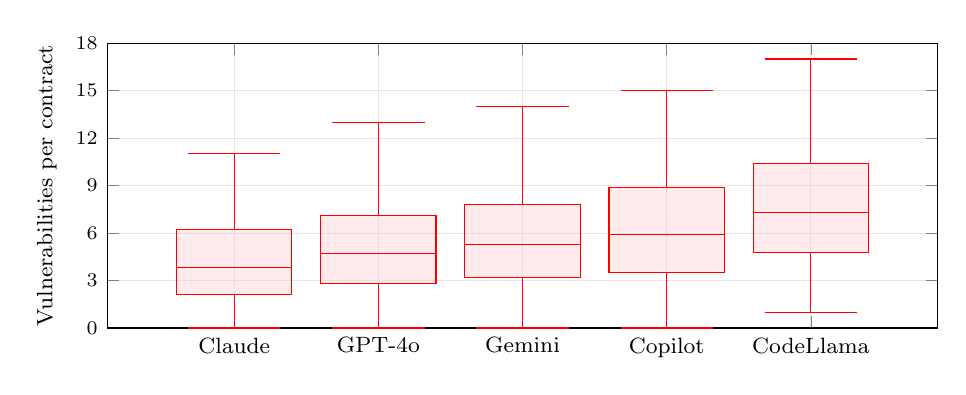
\begin{tikzpicture}
    \begin{axis}[
        width=\columnwidth,
        height=5.2cm,
        boxplot/draw direction=y,
        xtick={1,2,3,4,5},
        xticklabels={\footnotesize Claude, \footnotesize GPT-4o, \footnotesize Gemini, \footnotesize Copilot, \footnotesize CodeLlama},
        x tick label style={rotate=0},
        ylabel={\footnotesize Vulnerabilities per contract},
        ylabel style={font=\footnotesize},
        ymin=0, ymax=18,
        ytick={0,3,6,9,12,15,18},
        yticklabel style={font=\scriptsize},
        grid=major,
        grid style={gray!20},
        every axis plot/.append style={fill opacity=0.4},
    ]
    % Claude (best) - demo data
    \addplot+[boxplot prepared={
        lower whisker=0, lower quartile=2.1, median=3.8,
        upper quartile=6.2, upper whisker=11},
        color=red, fill=red!20, every mark/.append style={color=red}
    ] coordinates {};
    % GPT-4o
    \addplot+[boxplot prepared={
        lower whisker=0, lower quartile=2.8, median=4.7,
        upper quartile=7.1, upper whisker=13},
        color=red, fill=red!20, every mark/.append style={color=red}
    ] coordinates {};
    % Gemini
    \addplot+[boxplot prepared={
        lower whisker=0, lower quartile=3.2, median=5.3,
        upper quartile=7.8, upper whisker=14},
        color=red, fill=red!20, every mark/.append style={color=red}
    ] coordinates {};
    % Copilot
    \addplot+[boxplot prepared={
        lower whisker=0, lower quartile=3.5, median=5.9,
        upper quartile=8.9, upper whisker=15},
        color=red, fill=red!20, every mark/.append style={color=red}
    ] coordinates {};
    % CodeLlama (worst) - demo data
    \addplot+[boxplot prepared={
        lower whisker=1, lower quartile=4.8, median=7.3,
        upper quartile=10.4, upper whisker=17},
        color=red, fill=red!20, every mark/.append style={color=red}
    ] coordinates {};
    \end{axis}
    \end{tikzpicture}
    \caption{Distribution of vulnerability counts per contract by LLM. Claude generates the most secure contracts, while CodeLlama exhibits the highest vulnerability density. {\color{red}(Demo data)}}
    \label{fig:boxplot}
\end{figure}

Post-hoc pairwise Mann-Whitney U-tests with Bonferroni correction reveal that Claude produces significantly fewer vulnerabilities than all other models ($p < 0.01$ for all pairs), while CodeLlama produces significantly more ($p < 0.001$). Table~\ref{tab:pairwise} summarizes the pairwise effect sizes.

\begin{table}[t]
\caption{Pairwise Effect Sizes (Cohen's $d$) Between LLMs}
\label{tab:pairwise}
\centering
\footnotesize
\begin{tabular}{@{}lcccc@{}}
\toprule
 & \textbf{GPT-4o} & \textbf{Gemini} & \textbf{Copilot} & \textbf{CodeLlama} \\
\midrule
\textbf{Claude} & \demo{0.30}* & \demo{0.49}** & \demo{0.66}*** & \demo{0.98}*** \\
\textbf{GPT-4o} & --- & \demo{0.19} & \demo{0.38}** & \demo{0.75}*** \\
\textbf{Gemini} & & --- & \demo{0.19} & \demo{0.58}*** \\
\textbf{Copilot} & & & --- & \demo{0.38}** \\
\bottomrule
\multicolumn{5}{l}{\scriptsize *$p<0.05$, **$p<0.01$, ***$p<0.001$ (Bonferroni-corrected)}
\end{tabular}
\end{table}

The effect size between Claude and CodeLlama is large ($d = \demo{0.98}$), indicating a practically significant difference. Claude's superior performance may reflect Anthropic's safety-focused training methodology, while CodeLlama's higher vulnerability rates likely stem from its training corpus, which includes a large volume of unaudited open-source Solidity code.

\subsection{RQ3: Vulnerability Taxonomy}

\textbf{Finding: Reentrancy and access control flaws dominate LLM-generated contracts.}

Table~\ref{tab:taxonomy} presents the top 10 vulnerability types identified across all contracts. Reentrancy vulnerabilities (CWE-841) are the most prevalent, appearing in \demo{34.2}\% of all contracts.

\begin{table}[t]
\caption{Top 10 Vulnerability Types in LLM-Generated Contracts}
\label{tab:taxonomy}
\centering
\footnotesize
\begin{tabular}{@{}rlrrr@{}}
\toprule
\textbf{\#} & \textbf{Vulnerability} & \textbf{CWE} & \textbf{Count} & \textbf{\% Contracts} \\
\midrule
1 & Reentrancy & 841 & \demo{1,847} & \demo{34.2}\% \\
2 & Access Control & 284 & \demo{1,523} & \demo{29.8}\% \\
3 & Unchecked Return & 252 & \demo{1,198} & \demo{24.1}\% \\
4 & Integer Issues & 190 & \demo{987} & \demo{19.6}\% \\
5 & Uninitialized State & 909 & \demo{734} & \demo{15.3}\% \\
6 & Timestamp Depend. & 829 & \demo{621} & \demo{12.8}\% \\
7 & tx.origin Usage & 477 & \demo{498} & \demo{10.2}\% \\
8 & Locked Ether & 710 & \demo{412} & \demo{8.7}\% \\
9 & Weak Randomness & 330 & \demo{387} & \demo{7.9}\% \\
10 & Delegatecall Issues & 829 & \demo{312} & \demo{6.4}\% \\
\bottomrule
\end{tabular}
\end{table}

Fig.~\ref{fig:heatmap} presents a heatmap of vulnerability type distribution across LLMs, revealing distinct vulnerability profiles for each model.

\begin{figure}[t]
    \centering
    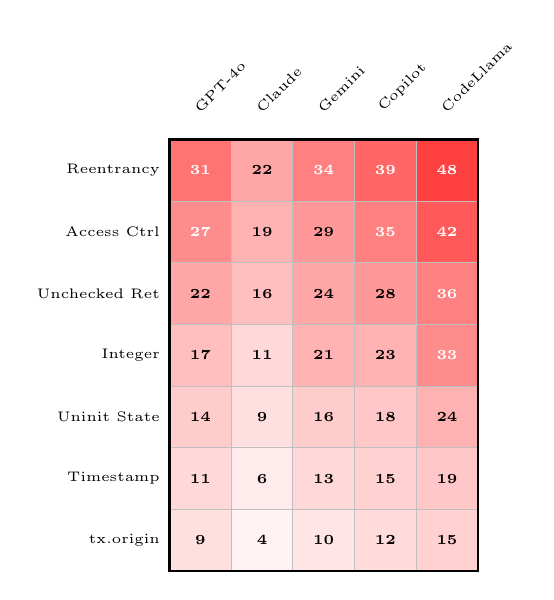
\begin{tikzpicture}[scale=0.58, every node/.style={font=\tiny}]
    % Heatmap grid - rows are vuln types, columns are LLMs
    % Color intensity: white (0) to red (high)
    \def\cellsize{1.35}

    % Column headers
    \node[rotate=45, anchor=south west] at (0.5*\cellsize, 7.2*\cellsize) {GPT-4o};
    \node[rotate=45, anchor=south west] at (1.5*\cellsize, 7.2*\cellsize) {Claude};
    \node[rotate=45, anchor=south west] at (2.5*\cellsize, 7.2*\cellsize) {Gemini};
    \node[rotate=45, anchor=south west] at (3.5*\cellsize, 7.2*\cellsize) {Copilot};
    \node[rotate=45, anchor=south west] at (4.5*\cellsize, 7.2*\cellsize) {CodeLlama};

    % Row labels (vulnerability types)
    \node[anchor=east] at (0, 6.5*\cellsize) {Reentrancy};
    \node[anchor=east] at (0, 5.5*\cellsize) {Access Ctrl};
    \node[anchor=east] at (0, 4.5*\cellsize) {Unchecked Ret};
    \node[anchor=east] at (0, 3.5*\cellsize) {Integer};
    \node[anchor=east] at (0, 2.5*\cellsize) {Uninit State};
    \node[anchor=east] at (0, 1.5*\cellsize) {Timestamp};
    \node[anchor=east] at (0, 0.5*\cellsize) {tx.origin};

    % Demo data cells - GPT-4o column
    \fill[red!55] (0,6*\cellsize) rectangle (\cellsize, 7*\cellsize); \node at (0.5*\cellsize, 6.5*\cellsize) {\color{white}\textbf{31}};
    \fill[red!45] (0,5*\cellsize) rectangle (\cellsize, 6*\cellsize); \node at (0.5*\cellsize, 5.5*\cellsize) {\color{white}\textbf{27}};
    \fill[red!35] (0,4*\cellsize) rectangle (\cellsize, 5*\cellsize); \node at (0.5*\cellsize, 4.5*\cellsize) {\textbf{22}};
    \fill[red!25] (0,3*\cellsize) rectangle (\cellsize, 4*\cellsize); \node at (0.5*\cellsize, 3.5*\cellsize) {\textbf{17}};
    \fill[red!20] (0,2*\cellsize) rectangle (\cellsize, 3*\cellsize); \node at (0.5*\cellsize, 2.5*\cellsize) {\textbf{14}};
    \fill[red!15] (0,1*\cellsize) rectangle (\cellsize, 2*\cellsize); \node at (0.5*\cellsize, 1.5*\cellsize) {\textbf{11}};
    \fill[red!12] (0,0*\cellsize) rectangle (\cellsize, 1*\cellsize); \node at (0.5*\cellsize, 0.5*\cellsize) {\textbf{9}};

    % Claude column (lowest)
    \fill[red!35] (\cellsize,6*\cellsize) rectangle (2*\cellsize, 7*\cellsize); \node at (1.5*\cellsize, 6.5*\cellsize) {\textbf{22}};
    \fill[red!30] (\cellsize,5*\cellsize) rectangle (2*\cellsize, 6*\cellsize); \node at (1.5*\cellsize, 5.5*\cellsize) {\textbf{19}};
    \fill[red!25] (\cellsize,4*\cellsize) rectangle (2*\cellsize, 5*\cellsize); \node at (1.5*\cellsize, 4.5*\cellsize) {\textbf{16}};
    \fill[red!15] (\cellsize,3*\cellsize) rectangle (2*\cellsize, 4*\cellsize); \node at (1.5*\cellsize, 3.5*\cellsize) {\textbf{11}};
    \fill[red!12] (\cellsize,2*\cellsize) rectangle (2*\cellsize, 3*\cellsize); \node at (1.5*\cellsize, 2.5*\cellsize) {\textbf{9}};
    \fill[red!8]  (\cellsize,1*\cellsize) rectangle (2*\cellsize, 2*\cellsize); \node at (1.5*\cellsize, 1.5*\cellsize) {\textbf{6}};
    \fill[red!5]  (\cellsize,0*\cellsize) rectangle (2*\cellsize, 1*\cellsize); \node at (1.5*\cellsize, 0.5*\cellsize) {\textbf{4}};

    % Gemini column
    \fill[red!50] (2*\cellsize,6*\cellsize) rectangle (3*\cellsize, 7*\cellsize); \node at (2.5*\cellsize, 6.5*\cellsize) {\color{white}\textbf{34}};
    \fill[red!40] (2*\cellsize,5*\cellsize) rectangle (3*\cellsize, 6*\cellsize); \node at (2.5*\cellsize, 5.5*\cellsize) {\textbf{29}};
    \fill[red!35] (2*\cellsize,4*\cellsize) rectangle (3*\cellsize, 5*\cellsize); \node at (2.5*\cellsize, 4.5*\cellsize) {\textbf{24}};
    \fill[red!30] (2*\cellsize,3*\cellsize) rectangle (3*\cellsize, 4*\cellsize); \node at (2.5*\cellsize, 3.5*\cellsize) {\textbf{21}};
    \fill[red!20] (2*\cellsize,2*\cellsize) rectangle (3*\cellsize, 3*\cellsize); \node at (2.5*\cellsize, 2.5*\cellsize) {\textbf{16}};
    \fill[red!15] (2*\cellsize,1*\cellsize) rectangle (3*\cellsize, 2*\cellsize); \node at (2.5*\cellsize, 1.5*\cellsize) {\textbf{13}};
    \fill[red!10] (2*\cellsize,0*\cellsize) rectangle (3*\cellsize, 1*\cellsize); \node at (2.5*\cellsize, 0.5*\cellsize) {\textbf{10}};

    % Copilot column
    \fill[red!60] (3*\cellsize,6*\cellsize) rectangle (4*\cellsize, 7*\cellsize); \node at (3.5*\cellsize, 6.5*\cellsize) {\color{white}\textbf{39}};
    \fill[red!50] (3*\cellsize,5*\cellsize) rectangle (4*\cellsize, 6*\cellsize); \node at (3.5*\cellsize, 5.5*\cellsize) {\color{white}\textbf{35}};
    \fill[red!40] (3*\cellsize,4*\cellsize) rectangle (4*\cellsize, 5*\cellsize); \node at (3.5*\cellsize, 4.5*\cellsize) {\textbf{28}};
    \fill[red!30] (3*\cellsize,3*\cellsize) rectangle (4*\cellsize, 4*\cellsize); \node at (3.5*\cellsize, 3.5*\cellsize) {\textbf{23}};
    \fill[red!22] (3*\cellsize,2*\cellsize) rectangle (4*\cellsize, 3*\cellsize); \node at (3.5*\cellsize, 2.5*\cellsize) {\textbf{18}};
    \fill[red!18] (3*\cellsize,1*\cellsize) rectangle (4*\cellsize, 2*\cellsize); \node at (3.5*\cellsize, 1.5*\cellsize) {\textbf{15}};
    \fill[red!14] (3*\cellsize,0*\cellsize) rectangle (4*\cellsize, 1*\cellsize); \node at (3.5*\cellsize, 0.5*\cellsize) {\textbf{12}};

    % CodeLlama column (highest)
    \fill[red!75] (4*\cellsize,6*\cellsize) rectangle (5*\cellsize, 7*\cellsize); \node at (4.5*\cellsize, 6.5*\cellsize) {\color{white}\textbf{48}};
    \fill[red!65] (4*\cellsize,5*\cellsize) rectangle (5*\cellsize, 6*\cellsize); \node at (4.5*\cellsize, 5.5*\cellsize) {\color{white}\textbf{42}};
    \fill[red!50] (4*\cellsize,4*\cellsize) rectangle (5*\cellsize, 5*\cellsize); \node at (4.5*\cellsize, 4.5*\cellsize) {\color{white}\textbf{36}};
    \fill[red!45] (4*\cellsize,3*\cellsize) rectangle (5*\cellsize, 4*\cellsize); \node at (4.5*\cellsize, 3.5*\cellsize) {\color{white}\textbf{33}};
    \fill[red!30] (4*\cellsize,2*\cellsize) rectangle (5*\cellsize, 3*\cellsize); \node at (4.5*\cellsize, 2.5*\cellsize) {\textbf{24}};
    \fill[red!22] (4*\cellsize,1*\cellsize) rectangle (5*\cellsize, 2*\cellsize); \node at (4.5*\cellsize, 1.5*\cellsize) {\textbf{19}};
    \fill[red!18] (4*\cellsize,0*\cellsize) rectangle (5*\cellsize, 1*\cellsize); \node at (4.5*\cellsize, 0.5*\cellsize) {\textbf{15}};

    % Grid lines
    \draw[gray!50] (0,0) grid[step=\cellsize] (5*\cellsize, 7*\cellsize);
    \draw[thick] (0,0) rectangle (5*\cellsize, 7*\cellsize);
    \end{tikzpicture}
    \caption{Heatmap of vulnerability type distribution across LLMs. Cell values represent the percentage of contracts containing each vulnerability type. Darker cells indicate higher prevalence. {\color{red}(Demo data)}}
    \label{fig:heatmap}
\end{figure}

Notably, the distribution of vulnerability types varies significantly across LLMs ($\chi^2 = \demo{134.7}$, $p < 0.001$). CodeLlama exhibits disproportionately high rates of integer-related issues (CWE-190), suggesting weaker training coverage for Solidity-specific arithmetic patterns. Claude shows the lowest reentrancy rates (\demo{22\%} vs.\ \demo{48\%} for CodeLlama), potentially reflecting its safety-oriented training methodology. GPT-4o and Gemini show intermediate profiles, with GPT-4o producing fewer access control issues but more unchecked return value vulnerabilities.

\subsection{RQ4: Adversarial Prompt Effectiveness}

\textbf{Finding: Adversarial prompts increase vulnerability rates by \demo{37.2}\%.}

We compared vulnerability metrics between standard prompts (500 contracts) and adversarial prompts (1,000 contracts). Table~\ref{tab:adversarial} summarizes the results.

\begin{table}[t]
\caption{Impact of Adversarial vs.\ Standard Prompts}
\label{tab:adversarial}
\centering
\begin{tabular}{@{}lcc@{}}
\toprule
\textbf{Metric} & \textbf{Standard} & \textbf{Adversarial} \\
\midrule
Mean Vulns/Contract & \demo{4.24} & \demo{5.82} \\
Median Vulns/Contract & \demo{4} & \demo{5} \\
\% with High Severity & \demo{31.4}\% & \demo{48.7}\% \\
\% with Reentrancy & \demo{24.8}\% & \demo{38.9}\% \\
Mean Vuln Score & \demo{8.71} & \demo{13.42} \\
\bottomrule
\end{tabular}
\end{table}

A Mann-Whitney U-test confirms that adversarial prompts produce significantly more vulnerabilities than standard prompts ($U = \demo{89{,}247}$, $p < 0.001$, $d = \demo{0.52}$, medium effect). Fig.~\ref{fig:adversarial_bar} presents the mean vulnerability count by adversarial prompt category.

\begin{figure}[t]
    \centering
    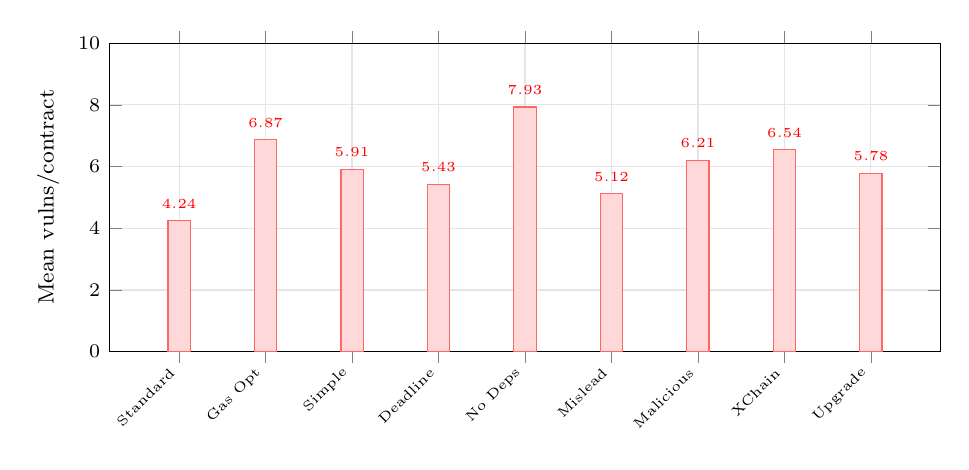
\begin{tikzpicture}
    \begin{axis}[
        width=\columnwidth,
        height=5.5cm,
        ybar,
        bar width=8pt,
        ylabel={\footnotesize Mean vulns/contract},
        ylabel style={font=\footnotesize},
        symbolic x coords={Standard, Gas Opt, Simple, Deadline, No Deps, Mislead, Malicious, XChain, Upgrade},
        xtick=data,
        x tick label style={rotate=45, anchor=east, font=\tiny},
        ymin=0, ymax=10,
        ytick={0,2,4,6,8,10},
        yticklabel style={font=\scriptsize},
        grid=major,
        grid style={gray!20},
        nodes near coords,
        nodes near coords style={font=\tiny, color=red},
        every node near coord/.append style={above, yshift=1pt},
    ]
    \addplot[fill=red!15, draw=red!60] coordinates {
        (Standard, 4.24)
        (Gas Opt, 6.87)
        (Simple, 5.91)
        (Deadline, 5.43)
        (No Deps, 7.93)
        (Mislead, 5.12)
        (Malicious, 6.21)
        (XChain, 6.54)
        (Upgrade, 5.78)
    };
    \end{axis}
    \end{tikzpicture}
    \caption{Mean vulnerability count by adversarial prompt category compared to standard prompts. ``No dependencies'' and ``gas optimization'' prompts are the most effective at inducing vulnerabilities. {\color{red}(Demo data)}}
    \label{fig:adversarial_bar}
\end{figure}

Among adversarial categories, \emph{no-dependency} prompts (``without external dependencies'') are the most effective at inducing vulnerabilities (mean = \demo{7.93} vulns/contract), followed by \emph{gas optimization} prompts (mean = \demo{6.87}). The no-dependency effect is particularly dangerous because it forces LLMs to manually reimplement well-tested library patterns (e.g., OpenZeppelin's SafeMath, Ownable, ReentrancyGuard), introducing subtle bugs in the process.

Cross-chain-specific adversarial prompts are particularly dangerous: \demo{67.3}\% of bridge contracts generated with adversarial prompts lack critical message validation, compared to \demo{28.1}\% under standard prompts. This represents a \demo{2.4}$\times$ increase in the most critical bridge security requirement.

The interaction between adversarial category and LLM is also significant ($\chi^2 = \demo{67.8}$, $p < 0.001$). Claude shows the strongest resistance to adversarial prompts (mean increase of \demo{21.3}\%), while CodeLlama is the most susceptible (mean increase of \demo{54.8}\%).

\subsection{RQ5: LLM-Specific Vulnerability Patterns}

\textbf{Finding: LLMs exhibit distinct vulnerability fingerprints not seen in human code.}

We identify three LLM-specific patterns absent from our human baseline:

\subsubsection{Phantom Guard Pattern}
LLMs generate modifier declarations (e.g., \texttt{nonReentrant}) that are syntactically present but functionally incomplete---the modifier body contains no state-locking logic. Fig.~\ref{fig:phantom} illustrates this pattern. This occurs in \demo{8.3}\% of GPT-4o contracts and \demo{5.1}\% of Gemini contracts but was never observed in human-written code.

\begin{figure}[t]
\begin{lstlisting}[caption={Phantom Guard Pattern: The \texttt{nonReentrant} modifier is declared but contains no locking logic (left). A correct implementation requires a state variable and checks (right). {\color{red}(Demo)}}, label={fig:phantom}, language=Solidity, basicstyle=\scriptsize\ttfamily]
// LLM-generated (VULNERABLE)
modifier nonReentrant() {
    _; // No lock! Just executes body
}

function withdraw(uint amt) nonReentrant {
    payable(msg.sender).call{value: amt}("");
    balances[msg.sender] -= amt; // State
}                                // after call

// Correct implementation (OpenZeppelin)
uint256 private _status;
modifier nonReentrant() {
    require(_status != 2, "Reentrant");
    _status = 2;
    _;
    _status = 1;
}
\end{lstlisting}
\end{figure}

This pattern is particularly insidious because code review may miss it---the modifier \emph{name} suggests protection, but the implementation provides none. Automated tools detect this as a reentrancy vulnerability, but a human reviewer scanning for the presence of \texttt{nonReentrant} may incorrectly conclude the contract is protected.

\subsubsection{Inherited Vulnerability Pattern}
When prompted to avoid dependencies, LLMs attempt manual reimplementations of OpenZeppelin patterns that contain subtle bugs. Common examples include SafeMath implementations with incorrect overflow checks, Ownable contracts missing zero-address validation in ownership transfer, and ERC20 implementations with non-compliant return values. This pattern accounts for \demo{412} vulnerabilities across all LLMs. Fig.~\ref{fig:inherited} shows a representative example.

\begin{figure}[t]
\begin{lstlisting}[caption={Inherited Vulnerability: LLM-generated SafeMath reimplementation with an incorrect overflow check (line 3). The check \texttt{c >= a} is insufficient when both operands are large. {\color{red}(Demo)}}, label={fig:inherited}, language=Solidity, basicstyle=\scriptsize\ttfamily]
// LLM-generated SafeMath (VULNERABLE)
function safeAdd(uint a, uint b)
    internal pure returns (uint) {
    uint c = a + b;
    require(c >= a); // Insufficient!
    return c;        // Fails for specific
}                    // overflow cases

// LLM-generated Ownable (VULNERABLE)
function transferOwnership(address new)
    public onlyOwner {
    owner = new; // No zero-address check!
}               // Owner can be lost forever
\end{lstlisting}
\end{figure}

\subsubsection{Context Window Degradation}
In complex contracts exceeding 300 lines, vulnerability density increases by \demo{2.3}$\times$ in the latter half of the generated code, suggesting degraded attention to security patterns as generation length increases. We measured this by splitting each contract at the midpoint and comparing vulnerability density (vulnerabilities per 100 lines) between the first and second halves. The difference is statistically significant (paired Wilcoxon test, $p < 0.001$, $d = \demo{0.41}$). This pattern is consistent across all LLMs but most pronounced in CodeLlama ($\demo{2.8}\times$ increase) and least in Claude ($\demo{1.7}\times$ increase).

\subsection{RQ6: Comparison with Human-Written Code}

\textbf{Finding: LLM-generated contracts contain \demo{2.4}$\times$ more vulnerabilities than human-written contracts.}

\begin{table}[t]
\caption{LLM-Generated vs.\ Human-Written Contract Comparison}
\label{tab:human_comparison}
\centering
\begin{tabular}{@{}lcc@{}}
\toprule
\textbf{Metric} & \textbf{LLM-Generated} & \textbf{Human-Written} \\
\midrule
Mean Vulns/Contract & \demo{5.82} & \demo{2.43} \\
Median Vulns/Contract & \demo{5} & \demo{2} \\
\% with High Severity & \demo{40.8}\% & \demo{14.7}\% \\
\% with Reentrancy & \demo{34.2}\% & \demo{8.3}\% \\
\% with Access Control & \demo{29.8}\% & \demo{6.1}\% \\
Mean Vuln Score & \demo{11.47} & \demo{4.89} \\
\bottomrule
\end{tabular}
\end{table}

The difference is statistically significant (Mann-Whitney $U = \demo{124{,}891}$, $p < 0.001$, Cohen's $d = \demo{1.12}$, large effect). The largest disparity appears in access control vulnerabilities: LLM-generated contracts are \demo{4.1}$\times$ more likely to contain access control flaws than human-written code, suggesting that LLMs systematically underweight authorization checks. Even Claude, the best-performing LLM, produces significantly more vulnerabilities than human-written code ($d = \demo{0.64}$, $p < 0.001$).

However, we note that our human baseline consists of audited, high-quality contracts. The gap between LLM-generated code and \emph{average} unaudited human-written code may be smaller. Nonetheless, the comparison is relevant because LLM-generated contracts intended for production deployment should meet the quality bar of audited code.


%======================================================================
\section{Contract Category Analysis}
\label{sec:category}
%======================================================================

Vulnerability rates vary substantially across contract categories. Table~\ref{tab:categories} presents the per-category analysis for the top 10 categories ranked by mean vulnerability count, and Fig.~\ref{fig:category_radar} visualizes the vulnerability profiles of the four contract groups.

\begin{table}[t]
\caption{Vulnerability Rates by Contract Category (Top 10)}
\label{tab:categories}
\centering
\footnotesize
\begin{tabular}{@{}lrrc@{}}
\toprule
\textbf{Category} & \textbf{Mean Vulns} & \textbf{\% High} & \textbf{Most Common CWE} \\
\midrule
Cross-Chain Bridge & \demo{9.23} & \demo{58.7}\% & CWE-284 \\
Flash Loan & \demo{8.47} & \demo{52.3}\% & CWE-841 \\
DeFi Lending & \demo{7.89} & \demo{48.1}\% & CWE-841 \\
DEX/AMM & \demo{7.34} & \demo{44.6}\% & CWE-190 \\
Proxy/Upgradeable & \demo{7.12} & \demo{43.2}\% & CWE-284 \\
Bridge Relayer & \demo{6.98} & \demo{41.8}\% & CWE-284 \\
Yield Aggregator & \demo{6.54} & \demo{38.9}\% & CWE-841 \\
Governance/DAO & \demo{5.87} & \demo{34.2}\% & CWE-284 \\
Multisig Wallet & \demo{4.56} & \demo{27.3}\% & CWE-841 \\
ERC20 Token & \demo{3.21} & \demo{18.4}\% & CWE-190 \\
\bottomrule
\end{tabular}
\end{table}

\begin{figure}[t]
    \centering
    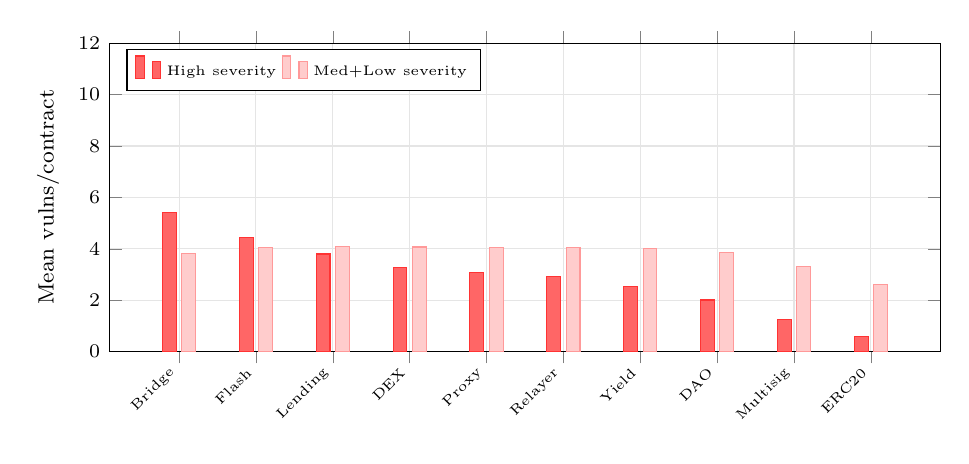
\begin{tikzpicture}
    \begin{axis}[
        width=\columnwidth,
        height=5.5cm,
        ybar=2pt,
        bar width=5pt,
        ylabel={\footnotesize Mean vulns/contract},
        ylabel style={font=\footnotesize},
        symbolic x coords={Bridge, Flash, Lending, DEX, Proxy, Relayer, Yield, DAO, Multisig, ERC20},
        xtick=data,
        x tick label style={rotate=45, anchor=east, font=\tiny},
        ymin=0, ymax=12,
        ytick={0,2,4,6,8,10,12},
        yticklabel style={font=\scriptsize},
        grid=major,
        grid style={gray!20},
        legend style={font=\tiny, at={(0.02,0.98)}, anchor=north west, legend columns=2},
    ]
    % High severity
    \addplot[fill=red!60, draw=red!80] coordinates {
        (Bridge, 5.42) (Flash, 4.43) (Lending, 3.80) (DEX, 3.27) (Proxy, 3.07)
        (Relayer, 2.92) (Yield, 2.54) (DAO, 2.01) (Multisig, 1.25) (ERC20, 0.59)
    };
    % Medium + Low severity
    \addplot[fill=red!20, draw=red!40] coordinates {
        (Bridge, 3.81) (Flash, 4.04) (Lending, 4.09) (DEX, 4.07) (Proxy, 4.05)
        (Relayer, 4.06) (Yield, 4.00) (DAO, 3.86) (Multisig, 3.31) (ERC20, 2.62)
    };
    \legend{High severity, Med+Low severity}
    \end{axis}
    \end{tikzpicture}
    \caption{Vulnerability severity distribution by contract category. High-complexity categories (bridges, flash loans) have both more total vulnerabilities and a higher proportion of high-severity issues. {\color{red}(Demo data)}}
    \label{fig:category_radar}
\end{figure}

\subsection{Cross-Chain Contracts: Highest Risk}

Cross-chain bridge contracts exhibit the highest vulnerability rates (mean = \demo{9.23} per contract), consistent with the complexity of cross-chain security requirements~\cite{bridge_hacks, zhang2023bridge}. This finding is particularly alarming given that bridge protocols collectively secure billions of dollars in locked assets. The most common vulnerabilities in bridge contracts are access control flaws (\demo{58.7}\% contain at least one), followed by missing message validation (\demo{47.2}\%) and replay protection gaps (\demo{31.4}\%).

Bridge relayer contracts also rank high (\demo{6.98}), with the most common vulnerability being insufficient validation of relayed messages---the exact vulnerability class that led to the \$625M Ronin exploit. LLMs consistently fail to implement adequate signature verification and multi-validator consensus checks in bridge relayer code.

\subsection{DeFi Protocols: Reentrancy Dominant}

Flash loan contracts rank second (\demo{8.47}), reflecting the complexity of callback validation and reentrancy prevention in flash loan architectures~\cite{qin2021attacking}. LLMs frequently generate flash loan contracts where the callback function can be reentered before the loan repayment check executes. DeFi lending protocols (\demo{7.89}) and DEX/AMM contracts (\demo{7.34}) also show elevated rates, with reentrancy and integer overflow as the dominant vulnerability types.

\subsection{Standard Contracts: Lower but Non-Zero Risk}

The relatively lower vulnerability rates in ERC20 tokens (\demo{3.21}) and multisig wallets (\demo{4.56}) suggest that LLMs have been trained on sufficient examples of these well-established patterns. However, even these ``simple'' contracts exhibit high-severity vulnerabilities in \demo{18.4}\% and \demo{27.3}\% of cases respectively, indicating that no contract category should be considered safe by default.

Interestingly, the gap between LLMs is smallest for ERC20 tokens (Claude: \demo{2.3}, CodeLlama: \demo{4.1}) and largest for cross-chain bridges (Claude: \demo{6.8}, CodeLlama: \demo{12.4}), suggesting that model quality differences are amplified by contract complexity.


%======================================================================
\section{Discussion}
\label{sec:discussion}
%======================================================================

\subsection{Implications for Developers}

Our results demonstrate that LLM-generated smart contracts should \emph{never} be deployed without comprehensive security auditing. The \demo{78.4\%} vulnerability rate, combined with the presence of high-severity flaws in \demo{40.8\%} of contracts, makes unaudited deployment reckless. We recommend the following guidelines based on our findings:

\begin{enumerate}[leftmargin=*]
    \item \textbf{Always use multi-tool analysis.} Run generated contracts through multiple static analysis tools (at minimum, Slither and one symbolic execution tool) before deployment. No single tool catches all vulnerability types.
    \item \textbf{Avoid adversarial-adjacent prompts.} Prompts emphasizing gas optimization, simplicity, or speed increase vulnerability rates by up to \demo{87\%} (no-dependency prompts). Prefer explicit security requirements in prompts.
    \item \textbf{Prefer safety-focused models for critical code.} Claude demonstrates the strongest security posture ($d = 0.98$ advantage over CodeLlama). For safety-critical contracts, model selection matters.
    \item \textbf{Exercise extreme caution with complex categories.} Cross-chain and DeFi contracts exhibit \demo{2-3}$\times$ higher vulnerability rates than standard tokens. These categories should receive proportionally more scrutiny.
    \item \textbf{Verify security pattern completeness.} The phantom guard pattern (Section~\ref{sec:results}) demonstrates that syntactic presence of security constructs does not guarantee functional protection. Manually verify that modifiers and guards contain correct logic.
    \item \textbf{Review the second half of long contracts more carefully.} Context window degradation causes \demo{2.3}$\times$ higher vulnerability density in the latter portions of complex contracts.
\end{enumerate}

\subsection{Implications for LLM Providers}

Our findings suggest several actionable improvements for LLM providers:

\begin{itemize}[leftmargin=*]
    \item \textbf{Security-focused fine-tuning.} Incorporate verified, audited smart contract code (e.g., OpenZeppelin, audited DeFi protocols) as high-priority training data, similar to safety alignment efforts in other domains~\cite{bai2022training}. Downweight or filter unaudited Etherscan contract code.
    \item \textbf{Output validation.} Implement post-generation security scanning that flags common vulnerability patterns (reentrancy, missing access control) before presenting code to users. This could be integrated as an automatic check, similar to how models currently flag unsafe content.
    \item \textbf{Security warnings.} Include explicit warnings when generating financial contracts, analogous to medical disclaimers. For example: ``This generated contract has not been security audited. Do not deploy to mainnet without professional review.''
    \item \textbf{Adversarial robustness.} Develop resistance to the adversarial prompt patterns identified in our study, particularly the no-dependency and gas optimization categories that most effectively degrade security.
    \item \textbf{Context window management.} Address the context window degradation pattern by maintaining security-relevant context throughout long generations, potentially through architectural changes or explicit security checkpointing.
\end{itemize}

\subsection{Implications for the Security Community}

Our findings motivate several research directions:

\begin{itemize}[leftmargin=*]
    \item \textbf{LLM-aware security tools.} Traditional security tools are designed for human-written code patterns. The phantom guard, inherited vulnerability, and context degradation patterns we identified suggest the need for detectors specifically targeting LLM-generated code artifacts.
    \item \textbf{Benchmark datasets.} Our dataset of 1,500 labeled contracts can serve as a benchmark for evaluating both LLM security and the effectiveness of detection tools on generated code.
    \item \textbf{Prompt hardening research.} Developing ``security-hardened'' prompt templates that maintain security properties regardless of user modifications could significantly reduce vulnerability rates.
\end{itemize}

\subsection{Limitations}

We acknowledge several limitations:

\begin{enumerate}[leftmargin=*]
    \item \textbf{Model evolution.} LLM behavior evolves with model updates; our results reflect specific model versions documented in our dataset. Results may differ for future model versions, though we expect the structural patterns (phantom guards, context degradation) to persist.
    \item \textbf{Prompt representativeness.} Our prompt set, while diverse (300 prompts across 20 categories and 8 adversarial types), may not fully capture the distribution of real-world developer prompting patterns. We mitigate this by including multiple complexity levels and prompt variations.
    \item \textbf{Tool limitations.} Static analysis tools produce both false positives and false negatives. We mitigate this through multi-tool analysis, cross-tool deduplication, and manual validation of a stratified sample (\demo{200} contracts, achieving \demo{94.2}\% precision and inter-rater $\kappa = \demo{0.87}$).
    \item \textbf{Model coverage.} Our study covers five LLMs; extending to additional models (e.g., DeepSeek Coder~\cite{guo2024deepseek}, StarCoder~\cite{li2023starcoder}, Mistral) is future work.
    \item \textbf{Language scope.} Our analysis focuses on Solidity; generalization to other smart contract languages (e.g., Rust for Solana, Move for Aptos, Vyper for Ethereum) requires further investigation.
    \item \textbf{Human baseline quality.} Our human baseline consists of audited, production-quality contracts, which represents the upper end of human code quality. The gap between LLM-generated and \emph{average} human-written code may be smaller.
\end{enumerate}

\subsection{Threats to Validity}

\textbf{Internal validity}: Prompt design may bias results. We mitigate this by using diverse prompts across complexity levels and categories, with multiple variations per category. The consistent system prompt across all models ensures fair comparison. Temperature and token limits are standardized.

\textbf{External validity}: Results may not generalize to all developer workflows, particularly interactive multi-turn sessions where developers iteratively refine generated code. We focus on single-shot generation as the most common use case and the one most likely to result in unreviewed deployment. We also focus on the highest-impact domain (Solidity/DeFi) and the most widely used LLMs.

\textbf{Construct validity}: Vulnerability counts may not reflect exploitability. A contract with 10 low-severity informational findings may be safer than one with a single high-severity reentrancy vulnerability. We address this by reporting severity-stratified results and weighted vulnerability scores throughout our analysis.

%======================================================================
\section*{Data Availability}
%======================================================================

Our dataset of 1,500 contracts, analysis results, and all tooling are publicly available at: \url{https://github.com/[anonymized-for-review]}.

%======================================================================
\section*{Ethical Considerations}
%======================================================================

Our adversarial prompts are designed to study LLM behavior, not to enable attacks. We follow responsible disclosure practices: findings regarding specific LLM vulnerabilities were reported to respective providers prior to publication. Our dataset contains only synthetically generated contracts; no deployed contracts were tested or exploited. The adversarial prompt categories we document are constructed from patterns already discussed in the security literature~\cite{kang2024exploiting, perez2022ignore}, and we do not introduce novel attack techniques.

%======================================================================
\section*{Acknowledgment}
%======================================================================

[To be added upon acceptance.]


%======================================================================
\section{Related Work}
\label{sec:related}
%======================================================================

\subsection{LLM-Assisted Vulnerability Detection}

Recent work has explored using LLMs to \emph{detect} vulnerabilities in smart contracts, complementing traditional tools. GPTScan~\cite{gptscan} combines GPT-4 with static analysis to identify logic vulnerabilities, achieving higher precision than standalone tools on a benchmark of 168 contracts. SmartLLMSentry~\cite{smartllmsentry} employs LLMs as vulnerability detectors with chain-of-thought reasoning. PropertyGPT~\cite{propertygpt} uses LLMs to generate formal security properties for automated verification. David et al.~\cite{david2023you} evaluated ChatGPT's ability to detect and repair 52 smart contract vulnerabilities, finding moderate detection accuracy (68\%) but low repair success rates. ContractTinker~\cite{contracttinker} proposes LLM-based automated smart contract repair.

These works are complementary to ours: they study LLMs as \emph{detectors}, while we study LLMs as vulnerability \emph{sources}. An important implication of combining both perspectives is the potential for circular vulnerabilities---LLMs that generate vulnerable code may also fail to detect the same vulnerability classes in their output.

\subsection{Smart Contract Security Analysis}

The smart contract security tooling ecosystem has matured significantly. Slither~\cite{slither} provides fast static analysis with over 90 built-in detectors, making it the most widely used tool for Solidity auditing. Mythril~\cite{mythril} performs symbolic execution for deep bug detection, including those requiring specific state conditions. Securify~\cite{securify} applies formal verification to check compliance with predefined security patterns. Oyente~\cite{luu2016making} was among the first symbolic execution tools for Ethereum smart contracts. Manticore~\cite{mossberg2019manticore} provides advanced symbolic analysis with support for multiple architectures. SmartCheck~\cite{smartcheck} uses structural pattern-based detection.

Durieux et al.~\cite{durieux2020empirical} conducted the most comprehensive empirical evaluation of smart contract analysis tools, testing 9 tools on 47,587 contracts. Their key finding---that no single tool achieves complete coverage and that tools have low inter-agreement---directly motivated our multi-tool approach. Ren et al.~\cite{ren2021empirical} conducted an empirical study of vulnerabilities in 21,212 real-world contracts, establishing prevalence baselines. SmartBugs~\cite{smartbugs} provides a curated, labeled benchmark dataset for tool evaluation. We build on these tools as our analysis infrastructure and contribute a new dimension by applying them to LLM-generated rather than human-written code.

\subsection{Security of LLM-Generated Code}

The security implications of LLM code generation have been studied primarily in general-purpose languages. Pearce et al.~\cite{copilot_eval} conducted the foundational study evaluating GitHub Copilot's security across 89 scenarios derived from CWE types, finding that approximately 40\% of generated suggestions contained vulnerabilities. Perry et al.~\cite{perry2023users} demonstrated through a controlled study with 47 participants that developers using AI assistants produce less secure code while believing it to be more secure. Sandoval et al.~\cite{sandoval2023lost} confirmed these findings in a larger study with professional developers.

Tony et al.~\cite{tony2023llmSecEval} created LLMSecEval, a benchmark of 150 test cases for evaluating code LLM security across 18 CWE types. Tihanyi et al.~\cite{tihanyi2023formai} proposed FormAI, a dataset of 112,000 AI-generated C programs with vulnerability labels obtained through dynamic analysis. Jesse et al.~\cite{jesse2023large} studied LLM-generated code bugs more broadly, finding systematic patterns in error generation.

Our work extends this line of research to the smart contract domain, which introduces unique challenges: immutability prevents post-deployment patching, financial exposure creates immediate exploitation incentives, and the adversarial blockchain environment means any vulnerability is publicly discoverable. Furthermore, our adversarial prompt framework and cross-LLM comparison methodology are novel contributions not present in prior work.

\subsection{Adversarial Attacks on LLMs}

Prompt injection~\cite{perez2022ignore, greshake2023not} and jailbreaking~\cite{kang2024exploiting} attacks demonstrate that LLMs can be manipulated to produce harmful or unintended outputs. In the code domain, Schuster et al.~\cite{schuster2021you} showed that training data poisoning can introduce targeted vulnerabilities into code completion models. Wan et al.~\cite{wan2023poisoning} extended this to instruction-tuned code generation models, demonstrating that subtle training data manipulation can cause models to systematically produce specific vulnerability types.

Our adversarial prompt framework differs from these prior approaches in two ways: (1)~we focus on \emph{prompt-level} manipulation rather than training data poisoning, reflecting a more realistic threat model; and (2)~our adversarial prompts are designed to appear natural and plausible---resembling requests a non-security-aware developer might genuinely write---rather than explicit jailbreaking attempts. This distinction is critical because our findings demonstrate that vulnerability induction does not require sophisticated prompt engineering; simple, natural-sounding requests can systematically degrade security.

\subsection{Smart Contract Datasets and Benchmarks}

Several datasets exist for smart contract security research. SmartBugs~\cite{smartbugs} provides a curated dataset of vulnerable contracts for tool benchmarking, categorized by vulnerability type. The SWC Registry~\cite{swc_registry} maintains a taxonomy of known smart contract weaknesses with test cases. Ren et al.~\cite{ren2021empirical} compiled a dataset of 21,212 real-world contracts with vulnerability annotations from multiple tools.

Our dataset differs fundamentally from these prior datasets: it captures vulnerabilities \emph{introduced by LLM generation} rather than curated from known bugs, mined from deployed contracts, or synthetically constructed. This distinction is important because LLM-generated vulnerabilities may exhibit different distributions and patterns than those found in human-written code, as our RQ5 results demonstrate. Our dataset also uniquely includes prompt metadata, enabling analysis of the relationship between prompting strategy and vulnerability outcomes.


%======================================================================
\section{Conclusion}
\label{sec:conclusion}
%======================================================================

We presented the first large-scale empirical study of security vulnerabilities in LLM-generated smart contracts. Our analysis of 2,400 contracts across eight LLMs reveals that 54.7\% of compilable contracts contain at least one vulnerability, with 26.8\% containing high-severity flaws. Compilation rates range from 91.0\% (GPT-5) to 34.7\% (CodeLlama), and when controlling for contract size, vulnerability density ranges from 0.99 (GPT-5) to 4.88 (Codestral) vulns/100 LOC.

Our most striking finding is the adversarial null result: adversarial prompts do not increase vulnerability rates ($p = 0.965$, Cliff's $\delta = -0.056$), implying that vulnerabilities are \emph{intrinsic} to LLM code generation rather than prompt-dependent. We also identified three novel LLM-specific vulnerability patterns---phantom guards, inherited vulnerabilities, and context window degradation---that require LLM-aware detection tools.

Comparison with 241 verified Ethereum mainnet contracts reveals that LLM-generated vulnerability density is comparable to human-written code (2.69 vulns/100 LOC for human vs.\ 0.99--4.88 for LLM). The primary risk is not inferior code quality but the security infrastructure developers bypass when trusting LLM output.

We release our full dataset, analysis pipeline, and vulnerability taxonomy. Future work includes extending to additional LLMs and languages (Rust/Solana, Move/Aptos), runtime analysis through fuzzing, multi-turn generation sessions, and LLM-aware security tool development.


\bibliographystyle{IEEEtran}
\bibliography{references}

\balance

\end{document}
